\section{Beta distribution ($Beta(\alpha, \beta)$)}

\begin{table}[H]
    \hfill
    \begin{minipage}{0.45\linewidth}
        \begin{figure}[H]
            \centering
            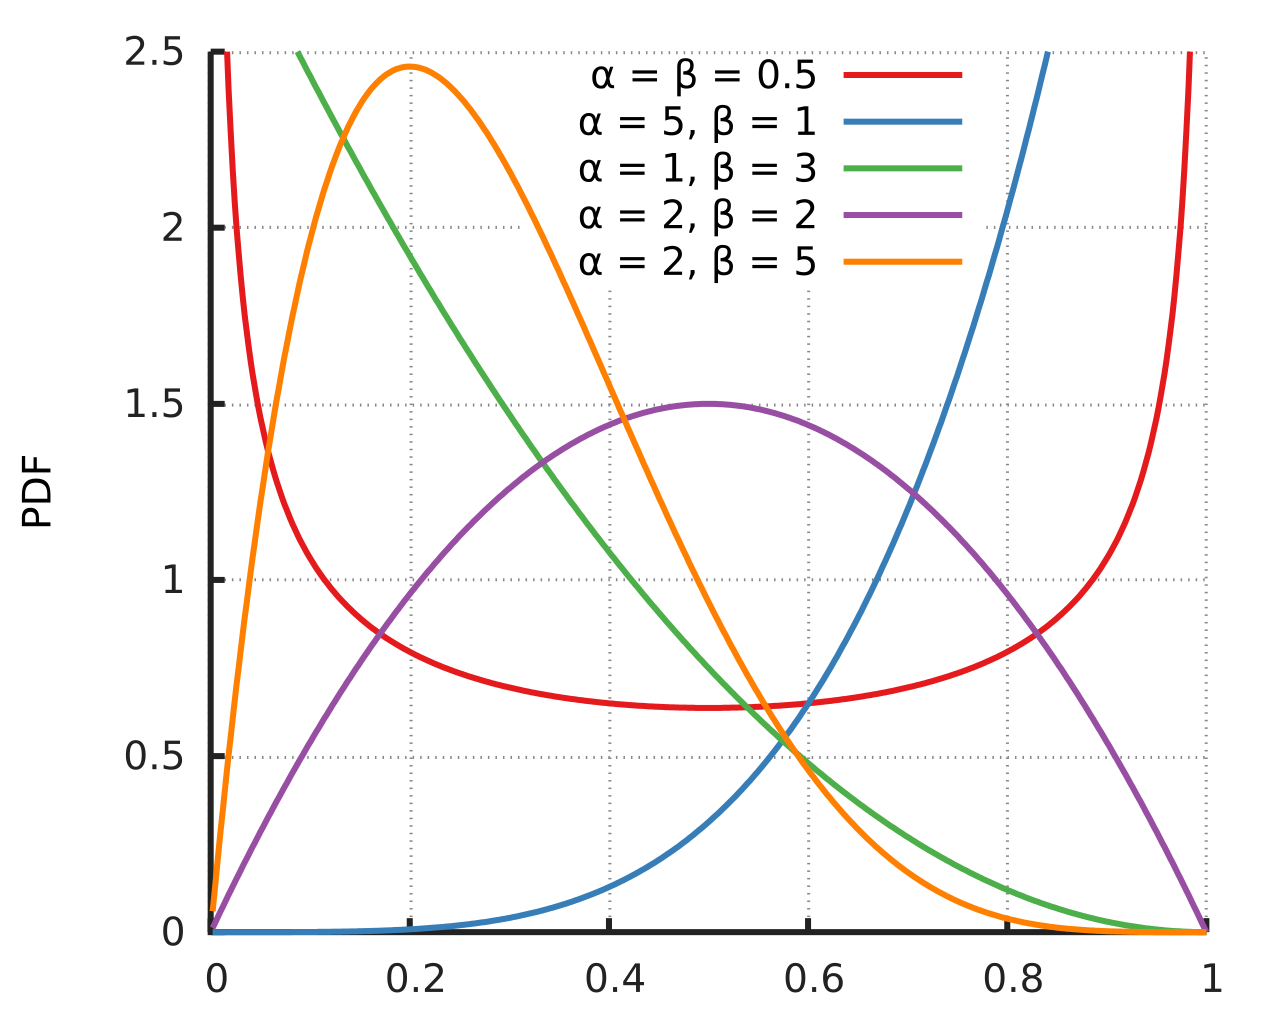
\includegraphics[
                width=\linewidth,
                height=5cm,
                keepaspectratio,
            ]{images/distributions/Beta_distribution_pdf.svg.png}
            \caption{Beta Distribution: PDF \cite{wiki/Beta_distribution}}
        \end{figure}
    \end{minipage}
    \hfill
    \begin{minipage}{0.45\linewidth}
        \begin{figure}[H]
            \centering
            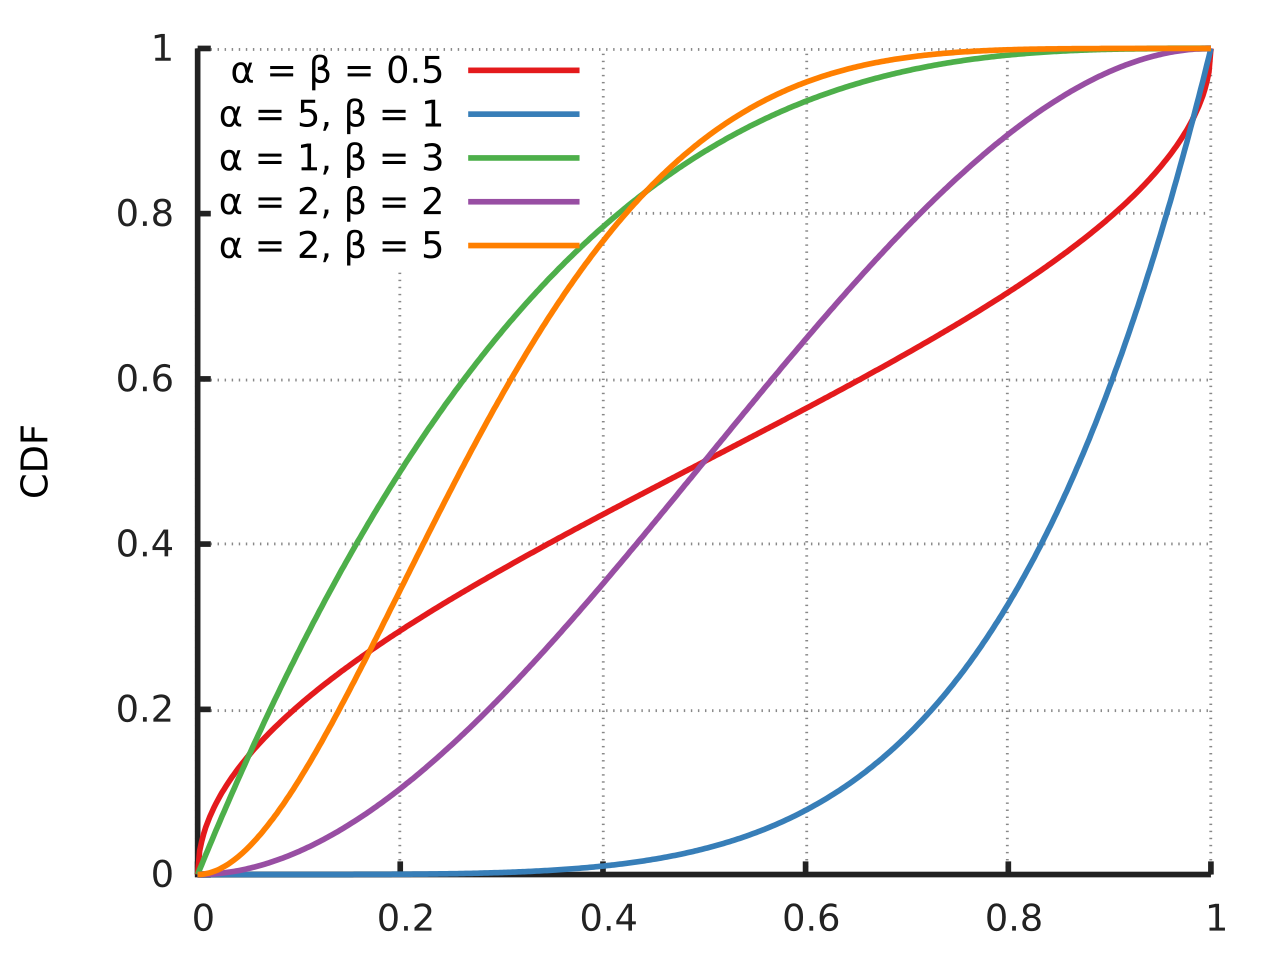
\includegraphics[
                width=\linewidth,
                height=5cm,
                keepaspectratio,
            ]{images/distributions/Beta_distribution_cdf.svg.png}
            \caption{Beta Distribution: CDF \cite{wiki/Beta_distribution}}
        \end{figure}
    \end{minipage}
    \hfill
\end{table}


\begin{enumerate}
    \item The beta distribution is considered a \textbf{conjugate prior distribution}.
    \hfill \cite{statistics/book/Statistics-for-Data-Scientists/Maurits-Kaptein}

    \item Intuitively, $\alpha$ moves probability mass toward $1$, whereas $\beta$ moves probability mass toward $0$.
    \hfill \cite{mfml/book/mml/Deisenroth-Faisal-Ong}
    \begin{enumerate}
        \item For $\alpha = 1 = \beta$, we obtain the \textbf{uniform distribution} $\mathcal{U}[0, 1]$.
        \hfill \cite{mfml/book/mml/Deisenroth-Faisal-Ong}

        \item For $\alpha, \beta < 1$, we get a \textbf{bimodal distribution} with spikes at $0$ and $1$.
        \hfill \cite{mfml/book/mml/Deisenroth-Faisal-Ong}

        \item For $\alpha, \beta > 1$, the distribution is \textbf{unimodal}.
        \hfill \cite{mfml/book/mml/Deisenroth-Faisal-Ong}

        \item For $\alpha, \beta > 1$ and $\alpha = \beta$, the distribution is \textbf{unimodal}, symmetric, and centered in the interval $[0, 1]$, i.e., the mode/mean is at $\dfrac{1}{2}$ .
        \hfill \cite{mfml/book/mml/Deisenroth-Faisal-Ong}
    \end{enumerate}
\end{enumerate}



\subsection{Summary}

\begin{enumerate}
    \item \textbf{Parameters}: 
    \begin{enumerate}
        \item $\alpha > 0$ shape (real)
        \hfill \cite{wiki/Beta_distribution}
        
        \item $\beta > 0$ shape (real)
        \hfill \cite{wiki/Beta_distribution}
    \end{enumerate}

    \item \textbf{Support}:  ${\displaystyle x\in [0,1]\!}$ or ${\displaystyle x\in (0,1)\!}$
    \hfill \cite{wiki/Beta_distribution}

    \item \textbf{PDF}:  ${\displaystyle {\dfrac {x^{\alpha -1}(1-x)^{\beta -1}}{\mathrm {B} (\alpha ,\beta )}}\!}$ 
    \hfill \cite{wiki/Beta_distribution}
    \\
    where ${\displaystyle \mathrm {B} (\alpha ,\beta )={\dfrac {\Gamma (\alpha )\ \Gamma (\beta )}{\Gamma (\alpha +\beta )}}}$ and ${\displaystyle \Gamma }$ is the \textbf{Gamma function}.
    \hfill \cite{wiki/Beta_distribution}

    \item \textbf{CDF}:  ${\displaystyle I_{x}(\alpha ,\beta )\!}$ (the regularized incomplete beta function)
    \hfill \cite{wiki/Beta_distribution}

    % \item \textbf{Quantile}: $  $
    % \hfill \cite{wiki/Beta_distribution}

    \item \textbf{Mean}:
    \begin{enumerate}
        \item ${\displaystyle \mbbE [X]={\dfrac {\alpha }{\alpha +\beta }}\!}$
        \hfill \cite{wiki/Beta_distribution}

        \item ${\displaystyle \mbbE[\ln X]=\psi (\alpha )-\psi (\alpha +\beta )\!}$
        \hfill \cite{wiki/Beta_distribution}

        \item ${\displaystyle \mbbE [X\,\ln X]={\dfrac {\alpha }{\alpha +\beta }}\,\left[\psi (\alpha +1)-\psi (\alpha +\beta +1)\right]\!}$
        \hfill \cite{wiki/Beta_distribution}
    \end{enumerate}
    where ${\displaystyle \psi }$ is the \textbf{digamma function}
    \hfill \cite{wiki/Beta_distribution}

    \item \textbf{Median}:  ${\displaystyle {\begin{matrix}I_{{1}/{2}}^{[-1]}(\alpha ,\beta ) \approx {\dfrac {\alpha -{{1}/{3}}}{\alpha +\beta -{{2}/{3}}}}{\text{ for }}\alpha ,\beta >1\end{matrix}}}$
    (in general)
    \hfill \cite{wiki/Beta_distribution}

    \item \textbf{Mode}: 
    ${\displaystyle {\dfrac {\alpha -1}{\alpha +\beta -2}}\!}$ for $\alpha, \beta > 1$
    \hfill \cite{wiki/Beta_distribution}
    \\
    Any value in the domain for $\alpha = \beta = 1$
    \hfill \cite{wiki/Beta_distribution}
    \\
    No mode if $\alpha<1$ or $\beta<1$. 
    Density diverges at 0 for $\alpha \leq 1$, and at 1 if $\beta \leq 1$
    \hfill \cite{wiki/Beta_distribution}

    \item \textbf{Variance}: 
    \begin{enumerate}
        \item 
        ${\displaystyle \mbbV [X]={\dfrac {\alpha \beta }{(\alpha +\beta )^{2}(\alpha +\beta +1)}}\!}$
        \hfill \cite{wiki/Beta_distribution}

        \item 
        ${\displaystyle \mbbV [\ln X]=\psi _{1}(\alpha )-\psi _{1}(\alpha +\beta )\!}$
        \hfill \cite{wiki/Beta_distribution}
    \end{enumerate}

    \item \textbf{Skewness}: $ {\displaystyle {\dfrac {2\,(\beta -\alpha ){\sqrt {\alpha +\beta +1}}}{(\alpha +\beta +2){\sqrt {\alpha \beta }}}}}$
    \hfill \cite{wiki/Beta_distribution}

    \item \textbf{Excess kurtosis}: $ {\displaystyle {\dfrac {6[(\alpha -\beta )^{2}(\alpha +\beta +1)-\alpha \beta (\alpha +\beta +2)]}{\alpha \beta (\alpha +\beta +2)(\alpha +\beta +3)}}}$
    \hfill \cite{wiki/Beta_distribution}

    \item \textbf{Entropy}: $   {\displaystyle {\begin{matrix}\ln \mathrm {B} (\alpha ,\beta )-(\alpha -1)\ \psi (\alpha )-(\beta -1)\ \psi (\beta )+(\alpha +\beta -2)\ \psi (\alpha +\beta )\end{matrix}}} $
    \hfill \cite{wiki/Beta_distribution}

    \item \textbf{Fisher information}: $  {\displaystyle {\begin{bmatrix}\mbbV  [\ln X]&\tCov [\ln X,\ln(1-X)]\\\tCov [\ln X,\ln(1-X)]&\mbbV  [\ln(1-X)]\end{bmatrix}}} $
    \hfill \cite{wiki/Beta_distribution}

    % \item \textbf{Expected shortfall}: $  $
    % \hfill \cite{wiki/Beta_distribution}

    \item \textbf{Moment-generating function (MGF)}: $   {\displaystyle 1+\sum _{k=1}^{\infty }\left(\prod _{r=0}^{k-1}{\dfrac {\alpha +r}{\alpha +\beta +r}}\right){\dfrac {t^{k}}{k!}}} $
    \hfill \cite{wiki/Beta_distribution}

    \item \textbf{Characteristic function (CF)}:
    $   {\displaystyle {}_{1}F_{1}(\alpha ;\alpha +\beta ;i\,t)\!}  $
    (see Confluent hypergeometric function)
    \hfill \cite{wiki/Beta_distribution}

    % \item \textbf{Probability-generating function (PGF)}: $  {\displaystyle (1-2\ln t)^{-k/2}{\text{ for }}0<t<{\sqrt {e}}\;} $
    % \hfill \cite{wiki/Beta_distribution}

    % \item \textbf{Kullback–Leibler divergence}:
    % $  $
    % \hfill \cite{wiki/Beta_distribution}

    \item \textbf{Method of moments}:
    \begin{enumerate}
        \item $  {\displaystyle \alpha =\left({\dfrac {E[X](1-E[X])}{V[X]}}-1\right)E[X]} $
        \hfill \cite{wiki/Beta_distribution}

        \item $  {\displaystyle \beta =\left({\dfrac {E[X](1-E[X])}{V[X]}}-1\right)(1-E[X])} $
        \hfill \cite{wiki/Beta_distribution}
    \end{enumerate}
\end{enumerate}




